\section{Reproducibility Summary}

%Add your summary here. No need to worry about fitting it in a single page now.
\section*{\centering Reproducibility Summary}

\textit{\citet{r1} gives a mathematically principled approach to solve the discrete optimization problem that occurs in the case of Binary Neural Networks and claims to give a similar performance on various classification benchmarks such as MNIST, CIFAR-10, and CIFAR-100 as compared to their full-precision counterparts, as well as other recent algorithms to train BNNs like PMF and Bop. The paper also claims that the BayesBiNN method has an application in the continual learning domain as it helps in overcoming catastrophic forgetting of the past by using the posterior approximation of the previous task as a prior for the upcoming task. We try to reproduce all the results presented in the original paper by making a separate and independent codebase.
}

\subsection*{Scope of Reproducibility}

We try to verify the performance of our re-implementation of the BayesBiNN optimizer on various classification and regression benchmarks. We also implemented the STE optimizer which was the central baseline model used in the paper. Finally, we tried to evaluate the results of BayesBiNN on the continual learning benchmark to get a better insight.

\subsection*{Methodology}

We developed our separate code-base, consisting of an end-to-end trainer with a Keras-like interface, for the reproduction which includes the implementation of the BayesBiNN and STE optimizer. We did refer to the author's code open-sourced on GitHub to get some insights about the hyperparameters and other doubts that emerged during code development.

\subsection*{Results}

We reproduced the accuracy of the BayesBiNN optimizer within less than 0.5\% of the originally reported value, which upholds the conclusion that it performs nearly as well as its full-precision counterpart in classification tasks. When we tried this in a semantic segmentation context, we found that the results were very underwhelming and in contrast with the seemingly good results by the STE optimizer even with much hyperparameter tuning. We can conclude that, like other Bayesian methods, it is difficult to train BayesBiNN on more complex tasks.

\subsection*{What was easy}

After we worked out the mathematics behind the BayesBiNN approach, we developed a pseudo-code for the optimization process which along with references from the author's code, helped us a lot in our reproduction study. 

\subsection*{What was difficult}

Some of the hyperparameters were not mentioned by the authors in their paper so it was difficult to approximate the values of those parameters. The lack of resources was the next big difficulty that we faced.

\subsection*{Communication with original authors}

We had a very fruitful conversation with the authors, which helped us in better understanding the BayesBiNN approach and its extension to the segmentation domain. The detailed pointers are given at the end of this report.

\subsection{Submission Checklist}

Double check the file \texttt{journal/metadata.yaml} to contain the following information:

\begin{itemize}
\item Title should start with "\texttt{[Re]}"
\item Author information, along with ORCID id
\item Author affiliations
\item Code URL, Software Heritage Foundation link
\item Abstract
\item Review URL (the OpenReview URL of your report)
\end{itemize}

\subsection{Continuous Integration}

We use Github Actions CI to check your submission and compile the pdf file subsequently.
You can also run the tests locally by running \texttt{python check\_yaml.py}, and then running \texttt{./build.sh} to compile Latex.

\clearpage

\section{Content}
Copy your Openreview content here.

This is an example citation \cite{Sinha:2021}.

\section{Introduction}

Most prominent vision datasets are afflicted by \emph{contextual bias}. For example, ``microwave" typically is found in kitchens, which also contain objects like ``refrigerator" and ``oven."  Such co-occurrence patterns may inadvertently induce contextual bias in datasets, which could consequently seep into models trained on them. When models overly rely on context, they may not generalize to settings where typical co-occurrence patterns are absent. The original paper by Singh et al.~\cite{Singh_2020_CVPR} proposes two methods for mitigating such contextual biases and improving the robustness of the learnt feature representations. The paper demonstrates their methods on multi-label object and attribute classification tasks, using the COCO-Stuff~\cite{caesar2018cvpr}, DeepFashion~\cite{liuLQWTcvpr16DeepFashion}, Animals with Attributes (AwA)~\cite{AwA}, and UnRel~\cite{Peyre17} datasets. Our exploration centers on four main directions:\\
\\
First, we trained the baseline classifier presented in the paper (Section~\ref{sec:baselineimplementation} for implementation and training details; Sections~\ref{sec:evaluation}-\ref{sec:baselineresults} for results). Due to likely implementation discrepancies, our results differed from the original paper by 0.6--3.1\% mAP on COCO-Stuff, by 0.7--1.4\% top-3 recall on DeepFashion, and by 0.1--3.2\% mAP on AwA (Table~\ref{tab:mainresults}). We ran a hyperparameter search (Appendix~\ref{sec:hyperparametersearch}), which yielded a significant (1.4--3.6\%) improvement on DeepFashion.\\
\\
Next, we identified the \emph{biased categories} in each dataset, i.e., visual categories that suffer from contextual bias. We followed the proposed method of using the baseline classifier to identify these categories, and discovered that the classifier implementation has a non-trivial effect. For COCO-Stuff, 18 of the top-20 categories we identified matched the original paper's top-20 categories (10 on DeepFashion, 18 on AwA; Section~\ref{sec:biasedcategories}). Nevertheless, the categories we identified appear reasonable  (e.g., ``fork" co-occurs with ``dining table"; Appendix~\ref{sec:biasedcategoriesapp}). As training and evaluation of most methods depend on the biased categories, we used the paper's biased categories for subsequent experiments.\\
\\
Third, we checked the main claim of the paper, that the proposed \emph{CAM-based} and \emph{feature-split} methods help improve recognition of biased categories in the absence of their context (Section~\ref{sec:stage2}). On COCO-Stuff, DeepFashion, and UnRel, we were able to reproduce the improvements gained from the proposed \textit{feature-split} method towards reducing contextual bias, whereas on AwA, we saw a drop in performance. The proposed \textit{CAM-based} method, which was only applied to COCO-Stuff, also helped reduce contextual bias, though not as significantly as the \textit{feature-split} method. For the  method, we reproduced the original paper's results to within 0.5\% mAP (Section~\ref{sec:mainresults}). We also successfully reproduced the paper's weight similarity analysis, as well as the qualitative analyses with class activation maps (CAMs)~\cite{zhou2015cnnlocalization}.\\
\\
Lastly, we ran additional experiments and ablation studies (Section~\ref{sec:addanalyses}). These revealed that the regularization term in the \emph{CAM-based} method and the weighted loss in the \emph{feature-split} method are central to the methods' performance. We also observed that varying the feature subspace size influences the \emph{feature-split} method's accuracy.

%%% SCOPE OF REPRODUCIBILITY %%%
\section{Scope of reproducibility} \label{sec:scope}

In this study, we aimed to verify the central claim of the original paper, which stated that the proposed algorithm outperforms other state-of-the-art approaches at calculating the truncated SVD of evolving matrices. In particular, they claimed that the method had especially high accuracy for the singular triplets with the largest modulus singular values. We sought to verify this claim by evaluating two metrics using our implementation of the method as well as with \verb|FrequentDirections|, a state-of-the-art matrix sketching and streaming algorithm \cite{Ghashami2016}:
\begin{enumerate}
    \item Relative approximation error \verb|rel_err| of leading $k$ singular values of $A$ (\Eqref{eq:rel_error}) is smaller when using the proposed algorithm compared to previous methods.
    \begin{equation}
        \verb|rel_err| = \abs{\dfrac{\hsigj{i}-\sigj{i}}{\sigj{i}}}
        \label{eq:rel_error}
    \end{equation}
    
    \item Scaled residual norm \verb|res_norm| of leading $k$ singular triplets $\{ \huj{i}, \hvj{i}, \hsigj{i} \}$ (\Eqref{eq:res_norm}) is smaller when using the proposed algorithm compared to previous methods.
    \begin{equation}
        \verb|res_norm| = \dfrac{\norm{A \hvj{i} - \hsigj{i} \huj{i}}_2}{\hsigj{i}}
        \label{eq:res_norm}
    \end{equation}
\end{enumerate}
Additionally, we also sought to verify the original paper's claims about the runtime performance of the proposed algorithm.

%%% PROJECTION-BASED UPDATE ALGORITHM %%%
\section{Projection-based update algorithm}
\label{sec:alg}

In the following sections, we first introduce the original \verb|zha-simon| algorithm, then introduce the proposed projection-based update algorithm.
Note that there are two implementations to the proposed algorithm: one which uses the same projection matrix as the \verb|zha-simon| algorithm (Algorithm 2.1) and another that uses an enhanced projection matrix (Algorithm 2.2).

%% ZHA-SIMON ALGORITHM %%
\subsection{Zha-Simon algorithm}
\label{alg:zha-simon}

As motivated in the introduction, an update algorithm that uses prior knowledge regarding the SVD of the matrix is crucial for it to be useful in practice.
The algorithm proposed in \cite{Kalantzis2021} is based on an algorithm proposed in \cite{Zha1999}, the latter of which we will refer to as the \verb+zha-simon+ algorithm (Algorithm \ref{alg:orig_zha-simon}).
Using \verb+zha-simon+ in the row-update case $A=\begin{pmatrix} B \\ E \end{pmatrix}$, the QR decomposition of the row space of $E$ that is not captured by the range of the right singular vectors $V_k$ can be expressed as $(I-V_k V_k^H)E^H = QR$.
Using this result and the previously known rank-$k$ SVD $B_k=U_k \Sigma_k V_k^H$, the updated matrix $A$ can be decomposed approximately as follows:
\begin{equation}
  A = \begin{pmatrix} B \\ E \end{pmatrix} \approx
  \begin{pmatrix} U_k \Sigma_k V_k^H \\ E \end{pmatrix} = 
  \begin{pmatrix} U_k & \\ & I_s \end{pmatrix} \begin{pmatrix} \Sigma_k & \\ EV_k & R^H \end{pmatrix} \begin{pmatrix} V_k^H \\ Q^H \end{pmatrix}
  \label{eq:zhasimon_partial}
\end{equation}
If we let $F\Theta G^H$ be the compact SVD of $\begin{pmatrix} \Sigma_k & \\ EV_k & R^H \end{pmatrix}$, then \Eqref{eq:zhasimon_partial} can be further decomposed as follows:
\begin{equation}
  A \approx 
  \begin{pmatrix} U_k & \\ & I_s \end{pmatrix} \left(F\Theta G^H\right) \begin{pmatrix} V_k^H \\ Q^H \end{pmatrix}
  = \left( \begin{pmatrix} U_k & \\ & I_s \end{pmatrix} F \right) \Theta \left( \begin{pmatrix} V_k & Q \end{pmatrix} G \right) ^H
  \label{eq:zhasimon_full}
\end{equation}
The key here is to notice that the approximation of the rank-$k$ truncated SVD of $A$ using the \verb+zha-simon+ algorithm does not require access to the previous matrix $B$ -- only the rank-$k$ SVD $B_k=U_k \Sigma_k V_k^H$ of the matrix from the previous iteration is needed.
We can further simplify \Eqref{eq:zhasimon_full} and see that it approximates the SVD of $A$ as $A \approx (ZF)\Theta(WG)^H$ where $Z=\begin{pmatrix} U_k & \\ & I_s \end{pmatrix}$ and $W^H=\begin{pmatrix} V_k & Q \end{pmatrix}^H$ are orthonormal matrices with ranges that approximately capture \verb+range+$(\hU_k)$ and \verb+range+$(\hV_k^H)$, respectively.

\begin{minipage}[t]{0.48\textwidth}
\begin{algorithm}[H]
    \centering
    \cprotect\caption{\verb|zha-simon| algorithm}\label{alg:orig_zha-simon}
    \begin{algorithmic}[1]
      \Require $A,E,U_k,\Sigma_k,V_k,k$
      \State $Z \gets \begin{pmatrix} U_k & \\ & I_s \end{pmatrix}$
      \State $[Q,R] \gets \verb|qr|(I-V_k V_k^H)E^H$ \label{op:zha-simon_qr}
      \State $W \gets \begin{pmatrix} V_k & Q \end{pmatrix}$
      \State $[F_k,\Theta_k,G_k] \gets \verb|svd|(Z^H AW,k)$ \label{op:zha-simon_svd}
      \State $\barU_k \gets Z F_k$
      \State $\barSigma_k \gets \Theta_k$
      \State $\barV_k \gets WG_k$
      \Ensure $\barU_k\approx\hU_k,\barSigma_k\approx\hSigma_k,\barV_k\approx\hV_k$
    \end{algorithmic}
\end{algorithm}
\end{minipage}
\hfill
\begin{minipage}[t]{0.48\textwidth}
\begin{algorithm}[H]
    \centering
    \caption{Proposed row-update algorithm} \label{alg:row-update}
    \begin{algorithmic}[1]
      \Require $B,E,k$
      \State $[U_k,\Sigma_k,V_k] \gets \verb|svd|(B,k)$
      \State Construct projection matrix $Z$
      \State $[F_k,\Theta_k] \gets \verb|svd|(Z^H A,k)$ where $A=\begin{pmatrix}B\\E\end{pmatrix}$ \label{op:row-update_svd}
      \State $\barU_k \gets Z F_k$
      \State $\barSigma_k \gets \Theta_k$
      \State $\barV_k \gets A^H \barU_k \barSigma_k^{-1}$
      \Ensure $\barU_k\approx\hU_k,\barSigma_k\approx\hSigma_k,\barV_k\approx\hV_k$
    \end{algorithmic}
\end{algorithm}
\end{minipage}

%% PROPOSED ALGORITHM %%
\subsection{Proposed row-update algorithm}

In practice, computing the rank-$k$ truncated SVD of $A$ using Algorithm \ref{alg:orig_zha-simon} is expensive due to the QR (Step \ref{op:zha-simon_qr}) and SVD (Step \ref{op:zha-simon_svd}) steps and possibly inaccurate based on the structure of $A$ \cite{Kalantzis2021}.
The cost of the QR decomposition can be mitigated by setting $W=I_n$ by observing that $\hv^{(i)}\subseteq\verb+range+(I_n)$ for $i=1,\dots,n$.
Therefore, $Z^H AW$ in Step \ref{op:zha-simon_svd} can be replaced with $Z^H A$ and the QR decomposition in Step \ref{op:zha-simon_qr} can be eliminated.
With these modifications, we have the new proposed row-update algorithm (Algorithm \ref{alg:row-update}).
Note that Step 2 has intentionally not been specified as the authors proposed two options for the construction of the projection matrix $Z$. 

The first option (Algorithm 2.1) uses the same $Z$ matrix as in Algorithm. Although the construction of $Z$ and $Z^H A$ are presented in two separate steps in Algorithm \ref{alg:row-update}, $Z^H A$ for Step \ref{op:row-update_svd} is directly computed as  \ref{alg:orig_zha-simon}. Below are the expressions for $Z$ and $Z^H A$ for Algorithm 2.1.
\begin{subequations}\label{eq:zha-simon_matrices}
\begin{equation}
  Z=\begin{pmatrix} U_k & \\ & I_s \end{pmatrix}
  \label{eq:zha-simon_Z}
\end{equation}
\begin{equation}
  Z^H A =
  \begin{pmatrix}
  \Sigma_k V_k^H \\
  E
  \end{pmatrix}
  \label{eq:zha-simon_ZHA}
\end{equation}
\end{subequations}


In the case where the rank of $B$ is larger than $k$ and the singular values $\sigma_{k+1},\dots,\sigma_{\text{min}(m,n)}$ are not small, the approximation returned by Algorithm 2.1 can be of poor accuracy.
Algorithm 2.2 addresses this by using an enhanced version of the projection matrix by adding a term $-B(\lambda) B E^H$ in the $Z$ matrix such that
\begin{equation}
  Z = \begin{pmatrix}
    U_k & -B(\lambda) B E^H & \\
    & & I_s
  \end{pmatrix}
\end{equation}
Setting $X = -B(\lambda) B E^H$, the additional term is equal to the matrix $X$ that satisfies the equation
\begin{equation}
    -(B B^H - \lambda I_m) X = (I_m - U_k U_k^H) B E^H,
    \label{eq:bcg}
\end{equation}
which can be computed using the block conjugate gradient (BCG) method \cite{OLeary1980}.
To ensure that the matrix $-(B B^H - \lambda I_m)$ is positive definite for BCG, a lower bound of $\lambda > \sigma_1^2$ is imposed.
The leading singular value can be estimated using a few iterations of truncated SVD.
However, to reduce the number of columns in $X$ and keep $Z$ manageable, the randomized rank-$r$ SVD of $X$ can be taken so that
\begin{equation}
    -B(\lambda) B E^H R \approx X_{\lambda,r} S_{\lambda,r} Y_{\lambda,r}^H
    \label{eq:bcg_rsvd}
\end{equation}
where $R$ is a matrix with at least $r$ columns whose entries are i.i.d.\ Gaussian random variables with zero mean and unit variance.
With $X_{\lambda,r}$, the $Z$ and $Z^H A$ matrices can be calculated as
\begin{subequations}
\begin{equation}
  Z = \begin{pmatrix}
    U_k & X_{\lambda,r} & \\
    & & I_s
  \end{pmatrix}
  \label{eq:enhanced_Z}
\end{equation}
\begin{equation}
  Z^H A =
  \begin{pmatrix}
    \Sigma_k V_k^H \\
    X_{\lambda,r}^H B \\
    E
  \end{pmatrix}
  \label{eq:enhanced_ZHA}
\end{equation}
\label{eq:enhanced_matrices}
\end{subequations}
For more detailed explanations and derivations of the algorithms and their associated proofs, we refer readers to \cite{Kalantzis2021}.

%%% METHODOLOGY %%%
\section{Methodology} \label{sec:methods}

Professor Vassilis Kalantzis, who we contacted via email, generously provided us with the relevant MATLAB code and data; however, we chose to re-implement the algorithm from scratch in Python with standard packages (NumPy \cite{numpy}, SciPy \cite{scipy}, and scikit-learn \cite{scikit-learn}) and used the MATLAB code to confirm our implementation. We compared the performance of Algorithms 2.1 and 2.2 with \verb|FrequentDirections| \cite{Ghashami2016}, a state-of-the-art streaming algorithm. Experiments were conducted on a MacBook Pro with a 2.3 GHz Dual-Core Intel Core i5 processor with 16 GB of RAM, and the code is publicly available on GitHub\footnote{https://anonymous.4open.science/r/truncatedSVD-0162/}. All plots were generated using Matplotlib \cite{matplotlib}.

%% IMPLEMENTATION
\subsection{Implementation}

We chose to implement the three truncated SVD update algorithms as methods of an \verb|EvolvingMatrix| class, which we will refer to as \verb|EM| from here on out. With each experiment, the \verb|EM| class was initialized with various parameters (initial matrix, matrix to be appended, number of batches, etc.) and updates were carried out using one of the update methods. A simplified version of the experiment is shown in Listing \ref{lst:exp_pseudo}. Algorithms 2.1 and 2.2 were written based on the pseudo-code presented in Algorithm \ref{alg:row-update}, where the $Z$ and $Z^H A$ matrices were calculated using their respective formulas. 

\lstinputlisting[language=python, float, floatplacement=h, caption=Simplified experiment structure, label={lst:exp_pseudo}]{sections/exp.py}

\paragraph{Algorithm 2.1}

The $Z$ and $Z^H A$ matrices were constructed as in Equations \ref{eq:zha-simon_Z} and \ref{eq:zha-simon_ZHA}, respectively. 

\paragraph{Algorithm 2.2}

The main difficulty in implementing Algorithm 2.2 was in the calculation of $X_{\lambda,r}$. We chose to solve for $X$ in Equation \ref{eq:bcg} using the block Conjugate Gradient method (BCG) \cite{OLeary1980} as recommended in \cite{Kalantzis2021}. Though \cite{Kalantzis2021} specified, at maximum, one iteration of BCG, we found that the MATLAB code set the limit to two iterations. As the additional iteration did not greatly increase the computational cost, we chose to run BCG a maximum of two iterations as well. Once $X$ was calculated, we calculated $X_{\lambda,r}$ as per Equation \ref{eq:bcg_rsvd} using randomized SVD \cite{Halko2011}. For this, we used the scikit-learn \verb|randomized_svd| implementation \cite{scikit-learn}. Based on the description for calculating $X_{\lambda,r}$ in \cite{Kalantzis2021}, we set \verb|n_components|$=r$, \verb|n_oversamples|$=2r$, and \verb|n_iter|$=0$. The $X_{\lambda,r}$ returned was then used to calculate $Z$ and $Z^H A$ as in Equations \ref{eq:enhanced_Z} and \ref{eq:enhanced_ZHA}, respectively.

\paragraph{Frequent Directions}

A modified version of \verb|FrequentDirections|\footnote{https://github.com/edoliberty/frequent-directions} was incorporated as an update method into the $\verb|EM|$ class.
Since \verb|FrequentDirections| is a line-by-line update method as opposed to a batch update method, the update method in the $\verb|EM|$ class was constructed to receive a matrix $E$ containing the rows to be added and performs the \verb|FrequentDirections| algorithms for each row of the $E$.
Any form of error metric calculation or subsequent update is performed only after the entire matrix $E$ has been processed using the line-by-line update method.

Since the updated matrix $B$ for the \verb|FrequentDirections| method has constant dimensions throughout the update process, the residual norm error calculation is modified to measure the error between $B$ and $A'$ where $A'$ is a truncated version of $A$ that only holds the first $2l$ singular vectors and values of $A$ and where $2l$ is the number of rows in $B$.

%% DATASETS %%
\subsection{Datasets}

In total, we conducted experiments on five datasets. MED, CRAN, CISI, and Reuters-21578 are term-document matrices from latent semantic indexing applications \cite{LSISite,Cai2005,Cai2007,Cai2008,Cai2009} and ML1M is a movie rating dataset from MovieLens \cite{Harper2015}. Table \ref{table:datasets} lists the dimensions of the matrices as well as the average number of nonzero (nnz) entries per row and Figure \ref{fig:sv} shows the leading 100 singular values for each matrix. It should be noted that the matrices used for CISI, CRAN, and MED in \cite{Kalantzis2021} had slightly different dimensions compared to what was listed on \cite{LSISite}. We received these datasets along with the MATLAB code and chose to use their versions of the data for ease of comparison; as we were interested in the accuracy of singular value reconstruction we determined that somewhat corrupted data merely introduced a different set of singular values to reconstruct. Furthermore, as the Reuters and ML1M datasets were intact, we used them as controls against the corruption of the other sets.

% Plot of singular value profile plot and table of data matrix stats
\begin{center}
\begin{minipage}[b]{0.4\textwidth}
% \begin{figure}[h]
  \centering
  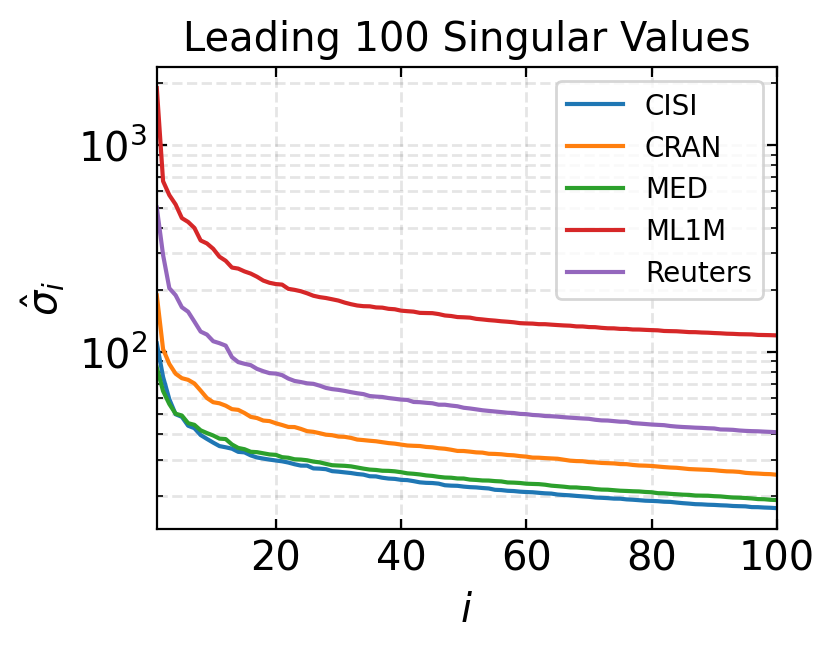
\includegraphics[width=0.9\textwidth]{figures/sv_100_profile.png}
  \captionof{figure}{Leading 100 singular values for each dataset.}
  \label{fig:sv}
% \end{figure}
\end{minipage}
\hfill
\begin{minipage}[b]{0.58\textwidth}
% \begin{table}[h]
  \centering
  \begin{tabular}{cccc}
    \toprule
    Dataset       & Rows  & Columns & nnz(A)/row \\
    \midrule
    CISI \cite{LSISite}                                     & 5609  &    1460 &      12.17 \\
    CRAN \cite{LSISite}                                     & 4612  &    1398 &      18.06 \\
    MED  \cite{LSISite}                                     & 5831  &    1033 &       8.92 \\
    ML1M \cite{Harper2015}                                  & 6040  &    3952 &     165.60 \\
    Reuters-21578 \cite{Cai2005, Cai2007, Cai2008, Cai2009} & 18933 &    8293 &      20.57 \\
    \bottomrule
    \vspace{5mm}
  \end{tabular}
  \\
  \captionof{table}{Number of rows, columns, and average non-zero elements in each row for datasets.}
  \label{table:datasets}
% \end{table}
\end{minipage}
\end{center}

%% EXPERIMENTS %%
\subsection{Experiments}

We conducted two sets of experiments: one to confirm the results of \cite{Kalantzis2021} in a series of reproducibility studies and another to further measure the performance of the algorithms using two additional metrics as well as observing the effect of the number of batches on the runtime and performance.

\paragraph{Update method comparison} 

As a first step, we sought to reproduce the results in Figures 3 and 4 of \cite{Kalantzis2021}. To do this, we conducted the sequence updates experiment. The initial matrix $B\equiv A^{(0)}$ was set equal to the first $\mu$ rows of $A\in\Ctwo{m}{n}$ and the remaining $m-\mu$ rows of $A$ were appended to the initial matrix over a sequence of $\phi$ updates, each with $\tau=\floor{(m-\mu)/\phi}$ rows. Following the notation of \cite{Kalantzis2021}, the $i$-th update would yield $A^{(i)} = \begin{pmatrix} B\equiv A^{(i-1)} \\ E\equiv A(\mu+(i-1)\tau+1:\mu+i\tau,:) \end{pmatrix}$ with the exception of the last update which is likely to have fewer rows in $E$. After each update, the rank-$k$ truncated SVD was calculated by one of the three algorithms.

The parameters used in \cite{Kalantzis2021}, and thus in our experiments as well were $\mu=\ceil{m/10}$ rows, $\phi=10$ updates, and rank $k=50$. The relative errors and residual norms were reported for the $k=50$ leading singular triplets for $\phi=1, 5, 10$. For Algorithm 2.2, we set the coefficient $\lambda=1.01 \hsigma_1^2$ and $r=10$.

\paragraph{Algorithm 2.2 $r$ parameter study}

Next, we varied the $r$ parameter in Algorithm 2.2 to evaluate its effect on the accuracy as was presented in Table 4 by \cite{Kalantzis2021}. For this, we set $\mu=\ceil{m/10}$, $\phi=10$, and $k=50$ for all three update methods as with the previous experiment and set $r=10,20,30,40,50$ for Algorithm 2.2.

\paragraph{Runtime comparison} 

We compared the runtimes of the algorithms for the CRAN, CISI, and MED as a function of the rank $k=25,25,50,75,100,125$ and the total number of updates $\phi=2,4,6,8,10$ (Figure 2 left and middle plots in \cite{Kalantzis2021}).

%\paragraph{Additional metrics}
%
%To further compare the performance of the algorithms, we additionally evaluated the accuracy of each method using the projection error \verb|proj_err|$=\norm{A-\hat{A}}_F^2 / \norm{A-A_k}_F^2$ and covariance error \verb|cov_err|=$\norm{A^T A-B^T B}_2 / \norm{A}_F^2$ introduced in \cite{Ghashami2016}.
%These two metrics were used in the \cite{Ghashami2016} to characterize the error between $B$ and $A$.
%
%For the projection error, $\hat{A}$ is defined as the rank $k$ matrix of the projection of $A$ onto $B$. Since $B$ is a subspace approximation of $A$, the projection will only retain the $2l$-dimensional subspace that contains the ``most common'' row space of $A$. Both the projection 
%
\paragraph{Varying number of batches and desired rank}

In addition to the experiments that we replicated based on \cite{Kalantzis2021}, we also varied the number of batches $\phi=2,4,6,8,10$ and the desired rank $k=25,50,75,100,125$ of the truncated SVD and evaluated the performance of each of the update methods to further observe the effects of each of these parameters on the methods' performances.

\section{Results}
In Table \autoref{tab:table1} we report our results for various classification benchmarks using our implemented BayesBiNN and STE optimizer. We notice that we get a difference of less than 0.1\% as compared to that in the original paper. We generated the results for baseline STE optimizer and full-precision networks by evaluating our implementation of these methods. We also generated the results of PMF, by modifying its original open-sourced code and using the hyperparameters mentioned in the original paper.

\begin{figure}[h]
     \centering
     \begin{subfigure}[b]{0.3\textwidth}
         \centering
         \includegraphics[width=1.2\textwidth]{../openreview/figs/MNIST.png}
         \caption{MNIST}
     \end{subfigure}
     \hfill
     \begin{subfigure}[b]{0.3\textwidth}
         \centering
         \includegraphics[width=1.2\textwidth]{../openreview/figs/CIFAR10.png}
         \caption{CIFAR10}
     \end{subfigure}
     \hfill
     \begin{subfigure}[b]{0.3\textwidth}
         \centering
         \includegraphics[width=1.2\textwidth]{../openreview/figs/CIFAR100.png}
         \caption{CIFAR100}
     \end{subfigure}
        \caption{Training/Validation/Test accuracy using BayesBiNN optimizer}
\end{figure}

\begin{table}[h]
\begin{center}
\begin{tabular}{ | c | c | c | c | c | }
\hline
 Datasets & Optimizer & Training Accuracy & Validation Accuracy & Test Accuracy \\ \hline
  \multirow{5}{4em}{MNIST} 
   & BayesBiNN(ours) & $99.90 \pm 0.01\%$ & $99.89 \pm 0.07\%$ & $98.87 \pm 0.06\%$  \\
   & BayesBiNN(orig.) & $99.85 \pm 0.05\%$ & $99.02 \pm 0.13\%$ & $98.86 \pm 0.05\%$  \\
   & STE & $99.90 \pm 0.01\%$ & $98.86 \pm 0.09\%$ & $98.89 \pm 0.05\%$  \\
   & PMF & - & $98.73\%$ & -  \\
   & Adam (Full Precision) & $99.98 \pm 0.01\%$ & $99.02 \pm 0.04\%$ & $99.02 \pm 0.01\%$  \\ 
\hline

  \multirow{5}{4em}{CIFAR10}
   & BayesBiNN(ours) & $99.96 \pm 0.01\%$ & $93.59 \pm 0.45\%$ & $93.54 \pm 0.26\%$  \\
   & BayesBiNN(orig.) & $99.96 \pm 0.01\%$ & $94.23 \pm 0.41\%$ & $93.72 \pm 0.16\%$  \\
   & STE & $99.99 \pm 0.01\%$ & $93.77 \pm 0.06\%$ & $93.54 \pm 0.08\%$  \\
   & PMF & - & $91.98\%$ & -  \\
   & Adam (Full Precision) & $99.99 \pm 0.01\%$ & $94.27 \pm 0.15\%$ & $94.38 \pm 0.16\%$  \\ 
\hline
   
   
  \multirow{5}{4em}{CIFAR100} 
   & BayesBiNN(ours) & $98.35 \pm 0.1\%$ & $74.13 \pm 0.78\%$ & $73.56 \pm 0.06 \%$ \\
   & BayesBiNN(orig.) & $98.02 \pm 0.18\%$ & $74.76 \pm 0.41\%$ & $73.68 \pm 0.31\%$  \\
   & STE & $99.22 \pm 0.03\%$ & $72.74 \pm 0.06\%$ & $73.25 \pm 0.26\%$  \\
   & PMF & - & $70.82\%$ & -  \\
   & Adam (Full Precision) & $99.89 \pm 0.02\%$ & $75.04 \pm 0.71\%$ & $74.80 \pm 0.39\%$  \\ \hline
\end{tabular}
\caption{Results of different optimizers trained on MNIST, CIFAR10, and CIFAR100.}
\label{tab:result_1}

\end{center}
\end{table}

\subsection{Comparison with LR-Net}
Authors compared their BayesBiNN approach to the LR-Net method presented in \citet{r8}. We tried to reproduce the result for the same setting. In this comparison, the data pre-processing and augmentation methods remain the same as mentioned in section 4.2, but we do not split the data in training and validation sets in this case. We denote the test accuracies after 190 epochs in the case of MNIST and 290 epochs in the case of CIFAR-10, as done in the original paper to maintain uniformity. Note that, our accuracy is matching with that of the original authors in the case of MNIST but not in the case of CIFAR-10. We suspect that this is due to some difference in Batch-Norm layers used.

\begin{table}[h]
\begin{center}
\renewcommand{\arraystretch}{1.1}
\begin{tabular}{ | c | c | c |}
\hline
 Optimizer & MNIST &  CIFAR10 \\ \hline
%   \multirow{2}{5em}{MNIST} 
   BayesBiNN (ours) & \textbf{99.52\%} & $84.49\%$ \\ \hline
   BayesBiNN (orig.) & $99.50\%$ & $\textbf{93.97\%}$ \\ \hline
   LR-net \citet{r8} & $99.47\%$ & $93.18\%$ \\
\hline
\end{tabular}
\caption{Test accuracy of BayesBiNN and LRNet.}
\label{tab:LR_result_2}

\end{center}
\end{table}

\subsection{Continual Learning}
As mentioned in the original paper, we try to reproduce the author's claims about weight distribution across tasks in a simple continual learning domain tested on Permuted MNIST. Clearly, as we learn across the tasks, the curve becomes flat from the middle conveying that the weights become more deterministic. Our result matches with the claims in the original paper.
\begin{figure}[h]
     \centering
     \begin{subfigure}[b]{0.3\textwidth}
         \centering
         \includegraphics[width=1.1\textwidth]{../openreview/figs/after_task_0.png}
         \caption{Prior $\lambda$}
     \end{subfigure}
     \hfill
     \begin{subfigure}[b]{0.3\textwidth}
         \centering
         \includegraphics[width=1.1\textwidth]{../openreview/figs/after_task_1.png}
         \caption{$\lambda$ after task 1}
     \end{subfigure}
     \hfill
     \begin{subfigure}[b]{0.3\textwidth}
         \centering
         \includegraphics[width=1.1\textwidth]{../openreview/figs/after_task_2.png}
         \caption{$\lambda$ after task 2}
     \end{subfigure}
        \caption{Distribution of $p(w=1)$ across consecutive learning tasks}
\end{figure}

\subsection{Visualization using Synthetic Dataset}

In the original paper, the authors present visualizations on binary classification (Two moons dataset\citet{r10}) and toy regression (Snelson dataset\citet{r9}) using STE and BayesBiNN optimizer. For the classification task, the authors claimed that STE is a more deterministic classifier compared to BayesBiNN. We reproduced this experiment and the results depicted in Figure \autoref{fig3} seem to be consistent with the author's claim. For the regression task, we conclude that the author's claim about BayesBiNN (mean) giving a smoother curve compared to STE is true, which can also be seen in Figure \autoref{fig4}. 


\begin{figure}[h]
     \centering
         \includegraphics[width=1\textwidth]{../openreview/figs/TwoMoon.png}
         \caption{Classification on Two Moons dataset using STE and BayesBiNN optimizer.}
         \label{fig3}
\end{figure}

\begin{figure}[h]
     \centering
         \includegraphics[width=0.6\textwidth]{../openreview/figs/Snelson.png}
         \caption{Regression on Snelson dataset using STE and BayesBiNN optimizer.}
         \label{fig4}
\end{figure}


\begin{table}[h]
\begin{center}
\setlength{\tabcolsep}{12pt}
\renewcommand{\arraystretch}{1.3}
\begin{tabular}{ | c | c | c | c | c | c | c | }
\hline
 \textbf{Temperature} & 10 & 1 & 0.1 & $10^{-2}$ & $10^{-3}$ & $10^{-4}$ \\\hline
 MSE Loss & 1.313 & 0.208 & 2.151 & 0.443 & 0.231 & 0.199\\ \hline
 \textbf{Temperature} & $10^{-5}$ & $10^{-6}$ & $10^{-7}$ & $10^{-8}$ & $10^{-9}$ & $10^{-10}$\\  \hline
 MSE Loss & 0.156 & 0.127 & 0.173 & 0.122 & 0.195 & 0.173\\ 
\hline
\end{tabular}
\caption{Mean square error loss of Snelson dataset for different temperatures.}
\label{tab:Ablation_result_4}

\end{center}
\end{table}

\subsection{Extended Results (Semantic Segmentation)}
We tried to validate the performance of the BayesBiNN optimizer on more complex tasks like semantic segmentation. Unfortunately, the results with BayesBiNN were quite underwhelming as compared to STE and its full-precision counterpart. We tried various parameters to improve its performance but none seemed to work. We had a brief discussion with the authors regarding this issue and the authors suggested that Bayesian models are intrinsically very difficult to train. For the results shown in Table \autoref{tab:table5} and Figure \autoref{fig5}, we have used the hyperparameters denoted in Table \autoref{tab:table1}.

\begin{table}[h]
\begin{center}
\renewcommand{\arraystretch}{1.1}
\begin{tabular}{ | c | c | c | c |}
\hline
  & BayesBiNN & STE &  Adam (Full Precision) \\ \hline
    Validation Score & 0.4102 & 0.3108 & 0.2943 \\ \hline
\end{tabular}
\caption{(1 - IoU) score for validation set}
\label{tab:table5}
\end{center}
\end{table}

\begin{figure}[h]
     \centering
     \begin{subfigure}[b]{0.3\textwidth}
         \centering
         \includegraphics[width=1.3\textwidth]{../openreview/figs/output_bayesbinn.png}
         \caption{BayesBiNN}
     \end{subfigure}
     \hfill
     \begin{subfigure}[b]{0.3\textwidth}
         \centering
         \includegraphics[width=1.3\textwidth]{../openreview/figs/output_ste.png}
         \caption{STE}
     \end{subfigure}
     \hfill
     \begin{subfigure}[b]{0.3\textwidth}
         \centering
         \includegraphics[width=1.3\textwidth]{../openreview/figs/output_normal.png}
         \caption{Adam}
     \end{subfigure}
        \caption{Some samples of segmented image outputs}
        \label{fig5}
\end{figure}
\section{Discussion}
\label{sec:disc}
% Give your judgement on if you feel the evidence you got from running the code supports the claims of the paper. Discuss the strengths and weaknesses of your approach - perhaps you didn't have time to run all the experiments, or perhaps you did additional experiments that further strengthened the claims in the paper.

% Summary
We were able to implement and train an Hamiltonian Generative Network with similar reconstruction performance of the ones of the original paper  ($30\%$ average absolute relative error wrt to their reported values when treating it as an autoencoder). These results show that the network is capable of exploiting the Hamiltonian equations to learn dynamics of a physical system from RGB images. However, the value of the resulting Hamiltonian does not remain constant throughout the system evolution. 
% \todo{Carles, Oleguer, check that what I write here makes sense}
This means that the network is learning something that is different from the Hamiltonian equations described in Section \ref{sec:data}.
%It is worth to note that there is an infinite number of equations whose partial derivatives in $q$ and $p$ match those of Eq. \ref{eq:hamilton}. In particular, a constant could be added to all Hamiltonian equations of Section \ref{sec:data} without changing the derivatives used by the integrators. Therefore, at each time-step the Hamiltonian network could predict any of these equations, explaining the high variance in the Hamiltonian values.   

To make the variational sampling work, we tried performing a grid search on the Geco\cite{geco} hyperparameters and using a fixed Lagrange multiplier as in \cite{beta-vae}. However, despite our best efforts, the samples produced by the variational model have very poor quality. This is generally due to the difficulty in minimizing both KL divergence and reconstruction loss. 

%To better evaluate the system, we provided further experiments giving a better grasp of the possibilities the Hamiltonian paradigm opens when using ANNs to learn about dynamical systems.
% Future work
We believe that further experiments are needed to understand better the behavior of the system and to improve it. Future work could include further testing on each network architecture, probably smaller networks would also be able to encode the needed information. Another next step is to try the approach on more challenging (and realistic-looking) environments. In addition, it would be interesting to tackle the transfer learning capabilities of such architecture between different environments. How re-usable each network is? How much faster the system is able to learn the new dynamics? Finally, another field which could benefit from this research is model-based reinforcement learning.
A generative approach from which to sample example rollouts could be very useful for training agents without the need of directly interacting with the environment.

\subsection{What was easy}
% Give your judgement of what was easy to reproduce. Perhaps the author's code is clearly written and easy to run, so it was easy to verify the majority of original claims. Or, the explanation in the paper was really easy to follow and put into code. 

% Be careful not to give sweeping generalizations. Something that is easy for you might be difficult to others. Put what was easy in context and explain why it was easy (e.g. code had extensive API documentation and a lot of examples that matched experiments in papers). 
Once we implemented the code it resulted quite easy to perform multiple experiments on different environments, architectures and hyper-parameters due to the code's modularity and flexibility.
We can define the the previously mentioned experiments and most common testing behaviors from a set of yaml files which can then be modified from command-line arguments.
While this required extra planning and work at the beginning it really payed off when debugging and evaluating in later stages. 

\subsection{What was difficult} \label{sec:challenge}
% List part of the reproduction study that took more time than you anticipated or you felt were difficult. 

% Be careful to put your discussion in context. For example, don't say "the maths was difficult to follow", say "the math requires advanced knowledge of calculus to follow". 

The main challenge we encountered is finding the correct tools to debug a model composed of so many interconnected networks.
The fact that it has a variational component with a dynamic Lagrange multiplier term makes it especially tricky to train.
Furthermore, no public implementation existed and some details and parameters were missing in the original paper leading to some necessary assumptions or parameter searches.


\subsection{Communication with original authors}
% Document the extent of (or lack of) communication with the original authors. To make sure the reproducibility report is a fair assessment of the original research we recommend getting in touch with the original authors. You can ask authors specific questions, or if you don't have any questions you can send them the full report to get their feedback before it gets published. 
We first tried to understand and re-implement the code by ourselves.
Nevertheless, at some point we had gathered a significant set of doubts and we decided to email them to the original authors, which they answered with great detail.
From that point onwards, we sent a couple more set of doubts, also receiving answers.\\

Most of our doubts were about network architecture clarifications (either of unclear or missing descriptions from the original paper), and loss function evaluation.
Furthermore, they provided us with some of their environment images so we could more easily make our environments as similar as possible.

\subsection{Improving reproducibility}
Having worked in re-implementing the whole original work, we feel it is important to share our experience as well as providing a recommendation on how it could be made more easily reproducible.
First, having the environments data or code to generate it available online would save the effort and, most importantly, it would constitute a baseline against which to compare future work.
Secondly, publishing all the hyperparameters and more details of the networks architecture would make the whole work much easier to reproduce and require less training attempts, especially for what concerns GECO.


\section*{Acknowledgements}
We thank Stathi Fotiadis for voluntarily contributing with a GECO \cite{geco} implementation draft to the public \href{https://github.com/CampusAI/Hamiltonian-Generative-Networks}{repo} and his useful feedback on code structuring. We thank the KTH Robotics, Perception, and Learning (RPL) Lab for the computational resources provided to us.
In addition, we would like to thank the original authors for providing further details on the implementation.
